\documentclass[aspectratio=169]{beamer}
\usetheme{Madrid}
\usepackage[utf8]{inputenc}
\usepackage[T1]{fontenc}
\usepackage[polish]{babel}
\usepackage{graphicx}
\usepackage{booktabs}
\usepackage{pgfplots}
\pgfplotsset{compat=1.18}
\usepgfplotslibrary{statistics}
\pgfplotsset{colormap={rylgn}{rgb255=(215,48,39) rgb255=(255,255,191) rgb255=(26,152,80)}}
\usetikzlibrary{arrows.meta}
\beamertemplatenavigationsymbolsempty

% --- dane figur współdzielone z raportem (06-report/figs) ---
\newcommand{\figpath}{../06-report/figs}

% --- Othello board helpers (TikZ); args = środek pola w jednostkach planszy ---
\definecolor{boardgreen}{RGB}{34,120,75}
\newcommand{\othbg}[2]{%
  \fill[boardgreen] (0,0) rectangle (#1,#2);
  \draw[black!45] (0,0) grid (#1,#2);
  \draw[black!85,very thick] (0,0) rectangle (#1,#2);}
\newcommand{\othB}[2]{\shade[ball color=black!82] (#1,#2) circle(0.34);
  \draw[black,thin] (#1,#2) circle(0.34);}
\newcommand{\othW}[2]{\shade[ball color=white] (#1,#2) circle(0.34);
  \draw[black!70,thin] (#1,#2) circle(0.34);}
\newcommand{\othcool}[2]{\draw[orange,line width=1.3pt] (#1,#2) circle(0.46);}
\newcommand{\othmove}[2]{\draw[black!85,dashed,line width=1pt] (#1,#2) circle(0.36);}
\newcommand{\othx}[2]{\draw[red,line width=1.3pt] (#1,#2) circle(0.42);
  \draw[red,line width=1.4pt] ({#1-0.25},{#2-0.25})--({#1+0.25},{#2+0.25});
  \draw[red,line width=1.4pt] ({#1-0.25},{#2+0.25})--({#1+0.25},{#2-0.25});}

% --- styl heatmapy współczynników wygranych ---
\pgfplotsset{
  heatmapaxis/.style={
    width=6.0cm, height=5.6cm, enlargelimits=false, axis on top,
    colormap name=rylgn, point meta min=0, point meta max=1,
    xtick={0,1,2,3,4,5},
    xticklabels={Random,Naive-Buro,Cooldown-Buro,UCT,UCT-PB-naive,UCT-PB-cooldown},
    ytick={0,1,2,3,4,5},
    yticklabels={Random,Naive-Buro,Cooldown-Buro,UCT,UCT-PB-naive,UCT-PB-cooldown},
    y dir=reverse,
    x tick label style={rotate=45,anchor=east,font=\tiny},
    y tick label style={font=\tiny},
    tick style={draw=none}, title style={font=\small},
  },
  heatlabels/.style={
    only marks, mark=none, point meta=explicit,
    nodes near coords={\pgfmathprintnumber[fixed,fixed zerofill,precision=2]{\pgfplotspointmeta}},
    every node near coord/.append style={font=\tiny,anchor=center,text=black},
  },
}
% --- styl boxplotów różnicy pionków ---
\pgfplotsset{marginaxis/.style={
  boxplot/draw direction=y, width=6.6cm, height=5.7cm,
  ymin=-39, ymax=39, xmin=0.3, xmax=6.7,
  xtick={1,2,3,4,5,6},
  xticklabels={Random,Naive-Buro,Cooldown-Buro,UCT,UCT-PB-naive,UCT-PB-cooldown},
  x tick label style={rotate=35,anchor=east,font=\tiny},
  ymajorgrids,
  ytick={-36,-24,-12,0,12,24,36}, y tick label style={font=\tiny},
  boxplot={box extend=0.55}, mark size=0.4pt, mark=o, title style={font=\small},
}}
\pgfplotsset{onebox/.style={boxplot, fill=blue!18, draw=blue!60!black,
  mark options={draw=blue!60!black}}}
\newcommand{\maxlines}{%
  \draw[densely dashed,red!70!black] (axis cs:0.3,36)--(axis cs:6.7,36);
  \draw[densely dashed,red!70!black] (axis cs:0.3,-36)--(axis cs:6.7,-36);
  \draw[gray!60] (axis cs:0.3,0)--(axis cs:6.7,0);}

\title[Cooldown Othello 6$\times$6]{MCTS/UCT w~grze Cooldown Othello 6$\times$6}
\author[W. Jasiński]{Wojciech Jasiński}
\institute[MSI2]{Metody Sztucznej Inteligencji 2}
\date{czerwiec 2026}

\begin{document}

\begin{frame}\titlepage\end{frame}

% --------------------------------------------------------------------
\begin{frame}{Gra: Othello 6$\times$6}
\textbf{Othello} -- deterministyczna gra dwuosobowa z~pełną informacją; ruch domyka linię pionków
przeciwnika i~odwraca je. Wygrywa gracz z~większą liczbą pionków. Gramy na planszy 6$\times$6
(zamiast 8$\times$8) -- mniejsza przestrzeń stanów pozwala na statystycznie wiarygodne porównania.
\vspace{2pt}
\begin{columns}[t]
\begin{column}{0.33\textwidth}\centering
\begin{tikzpicture}[scale=0.5]
\othbg{6}{6}
\othW{2.5}{3.5}\othB{3.5}{3.5}\othB{2.5}{2.5}\othW{3.5}{2.5}
\end{tikzpicture}\\[2pt]{\scriptsize pozycja startowa}
\end{column}
\begin{column}{0.33\textwidth}\centering
\begin{tikzpicture}[scale=0.5]
\othbg{6}{6}
\othB{1.5}{5.5}\othB{5.5}{5.5}
\othB{1.5}{4.5}\othB{2.5}{4.5}\othB{4.5}{4.5}
\othW{0.5}{3.5}\othB{1.5}{3.5}\othB{2.5}{3.5}\othB{3.5}{3.5}\othW{4.5}{3.5}
\othW{0.5}{2.5}\othW{1.5}{2.5}\othW{2.5}{2.5}\othW{3.5}{2.5}\othW{4.5}{2.5}
\othB{0.5}{1.5}\othW{1.5}{1.5}\othW{2.5}{1.5}\othW{4.5}{1.5}
\othB{0.5}{0.5}\othW{2.5}{0.5}\othW{4.5}{0.5}
\othmove{0.5}{4.5}\othmove{5.5}{3.5}\othmove{3.5}{1.5}\othmove{5.5}{1.5}\othmove{1.5}{0.5}\othmove{5.5}{0.5}
\end{tikzpicture}\\[2pt]{\scriptsize środek gry: legalne ruchy (\,\tikz\draw[black!85,dashed] (0,0) circle(0.08);\,)}
\end{column}
\begin{column}{0.33\textwidth}\centering
\begin{tikzpicture}[scale=0.5]
\othbg{6}{6}
\othB{0.5}{5.5}\othB{1.5}{5.5}\othW{2.5}{5.5}\othW{3.5}{5.5}\othW{4.5}{5.5}\othW{5.5}{5.5}
\othB{0.5}{4.5}\othB{1.5}{4.5}\othB{2.5}{4.5}\othB{3.5}{4.5}\othB{4.5}{4.5}\othW{5.5}{4.5}
\othB{0.5}{3.5}\othB{1.5}{3.5}\othB{2.5}{3.5}\othB{3.5}{3.5}\othB{4.5}{3.5}\othW{5.5}{3.5}
\othB{0.5}{2.5}\othB{1.5}{2.5}\othW{2.5}{2.5}\othB{3.5}{2.5}\othB{4.5}{2.5}\othW{5.5}{2.5}
\othB{0.5}{1.5}\othW{1.5}{1.5}\othW{2.5}{1.5}\othW{3.5}{1.5}\othW{4.5}{1.5}\othW{5.5}{1.5}
\othW{0.5}{0.5}\othW{1.5}{0.5}\othW{2.5}{0.5}\othW{3.5}{0.5}\othW{4.5}{0.5}\othW{5.5}{0.5}
\end{tikzpicture}\\[2pt]{\scriptsize koniec: partia człowiek--komputer, 19:17}
\end{column}
\end{columns}
\vspace{4pt}
\centering\small Zagraj online:
\href{https://wojtke.github.io/cooldown-othello-mcts}{\texttt{wojtke.github.io/cooldown-othello-mcts}}
\end{frame}

% --------------------------------------------------------------------
\begin{frame}{Reguła stygnięcia (Cooldown)}
\textbf{Autorska modyfikacja:} pionki postawione lub odwrócone w~poprzedniej turze są \emph{chronione}
przez jedną turę -- są \emph{przezroczyste}, nie można ich od razu odbić.
\begin{columns}[c]
\begin{column}{0.50\textwidth}
\begin{itemize}\small
  \item eliminuje \emph{whipsaw} (natychmiastowe odbicie tych samych pionków),
  \item wprowadza \emph{zależność od historii}: stan to para \texttt{(plansza, ostudzone)},
  \item osłabia tablice transpozycji i~klasyczne wagi pozycyjne,
  \item empirycznie (1000 partii losowych): rozgałęzienie 5,3$\to$4,5; długość gry $\approx$34--35
        półruchów w~obu wariantach.
\end{itemize}
\end{column}
\begin{column}{0.50\textwidth}\centering
\begin{tikzpicture}[scale=0.5]
\othbg{4}{3}
\othB{0.5}{1.5}\othW{1.5}{1.5}\othW{2.5}{1.5}\othW{1.5}{0.5}
\othmove{3.5}{1.5}\draw[-{Latex},thick,black] (3.2,1.5)--(1.05,1.5);
\end{tikzpicture}\;
\begin{tikzpicture}[scale=0.5]
\othbg{4}{3}
\othB{0.5}{1.5}\othB{1.5}{1.5}\othB{2.5}{1.5}\othB{3.5}{1.5}\othW{1.5}{0.5}
\othcool{1.5}{1.5}\othcool{2.5}{1.5}\othcool{3.5}{1.5}
\end{tikzpicture}\;
\begin{tikzpicture}[scale=0.5]
\othbg{4}{3}
\othB{0.5}{1.5}\othB{1.5}{1.5}\othB{2.5}{1.5}\othB{3.5}{1.5}\othW{1.5}{0.5}
\othcool{1.5}{1.5}\othx{1.5}{2.5}
\end{tikzpicture}
\\[3pt]{\scriptsize (a) bicie czarnego $\to$ (b) odwrócone pionki stygną
(\textcolor{orange}{$\circ$}) $\to$ (c) odbicie \textcolor{red}{nielegalne}}
\end{column}
\end{columns}
\end{frame}

% --------------------------------------------------------------------
\begin{frame}{Gracze i~hipotezy}
\textbf{6~graczy:} Random; Naive-Buro, Cooldown-Buro (heurystyki 1-warstwowe);
UCT; UCT-PB-naive, UCT-PB-cooldown (UCT + progressive bias).
\begin{block}{Hipotezy}
\begin{itemize}\small
  \item[H1] UCT $>$ heurystyki, mocniej pod regułą stygnięcia.
  \item[H2] Progressive bias z~Cooldown-Buro $>$ bazowy UCT o~$\geq$10~p.p.
  \item[H3] Cooldown-Buro $>$ Naive-Buro tylko pod regułą stygnięcia.
  \item[H4] Przewaga drugiego gracza zanika pod regułą stygnięcia.
\end{itemize}
\end{block}
\end{frame}

% --------------------------------------------------------------------
\begin{frame}{Metodologia}
\begin{itemize}
  \item Silnik gry i~MCTS napisane od zera (Python); eksperymenty zrównoleglone
        (maszyna 128~rdzeni, \texttt{multiprocessing}).
  \item Turniej round-robin: 15~par $\times$ 200~partii $\times$ 2~warianty $=$ 6000~partii,
        budżet $B=10\,000$ symulacji/ruch.
  \item Samogra najsilniejszego wariantu ($\geq$2000 partii) dla H4.
  \item Strojenie: Optuna~TPE, kaskadowo, $B_{\text{tune}}=2000$.
  \item Statystyka: przedziały Wilsona, test dwumianowy, McNemar, korekta Holma.
\end{itemize}
\end{frame}

% --------------------------------------------------------------------
\begin{frame}{Wyniki -- ranking}
\centering
\begin{tikzpicture}
\begin{axis}[ybar, bar width=8pt, width=0.86\textwidth, height=0.62\textheight,
  symbolic x coords={UCT-PB-cooldown,UCT-PB-naive,UCT,Cooldown-Buro,Naive-Buro,Random},
  xtick=data, x tick label style={rotate=20,anchor=east,font=\small},
  ymin=0, ymax=1, ylabel={śr.\ współczynnik wygranych}, ylabel style={font=\small},
  y tick label style={font=\small},
  legend pos=north east, legend style={font=\small},
  enlarge x limits=0.10, ymajorgrids, tick align=outside,
  nodes near coords, every node near coord/.append style={font=\tiny}]
\addplot[fill=blue!55] table[x=method,y=classic] {\figpath/ranking.dat};
\addplot[fill=red!60]  table[x=method,y=cooldown] {\figpath/ranking.dat};
\legend{klasyk,cooldown}
\end{axis}
\end{tikzpicture}\\
{\small MCTS $\gg$ heurystyki. UCT-PB-cooldown jako jedyny utrzymuje wysoki wynik w~\emph{obu}
wariantach (0,84/0,81); UCT-PB-naive załamuje się pod regułą (0,86$\to$0,64).}
\end{frame}

% --------------------------------------------------------------------
\begin{frame}{Wyniki -- współczynniki wygranych (para po parze)}
\centering
\resizebox{0.98\textwidth}{!}{%
\begin{tikzpicture}\begin{axis}[heatmapaxis, title={Klasyczne 6$\times$6}]
\addplot[matrix plot*, mesh/cols=6, mesh/ordering=rowwise, point meta=explicit]
  table[meta=c] {\figpath/heatmap_classic_grid.dat};
\addplot[heatlabels] table[meta=c] {\figpath/heatmap_classic_lab.dat};
\end{axis}\end{tikzpicture}%
\hspace{4pt}%
\begin{tikzpicture}\begin{axis}[heatmapaxis, title={Cooldown 6$\times$6}, yticklabels={}, ylabel={},
  colorbar, colorbar style={width=0.18cm,font=\tiny}]
\addplot[matrix plot*, mesh/cols=6, mesh/ordering=rowwise, point meta=explicit]
  table[meta=c] {\figpath/heatmap_cooldown_grid.dat};
\addplot[heatlabels] table[meta=c] {\figpath/heatmap_cooldown_lab.dat};
\end{axis}\end{tikzpicture}}\\
{\small Wartość = odsetek wygranych gracza z~wiersza przeciw graczowi z~kolumny.}
\end{frame}

% --------------------------------------------------------------------
\begin{frame}{Strojenie: zależność celu od~$c$ (PDP)}
\centering
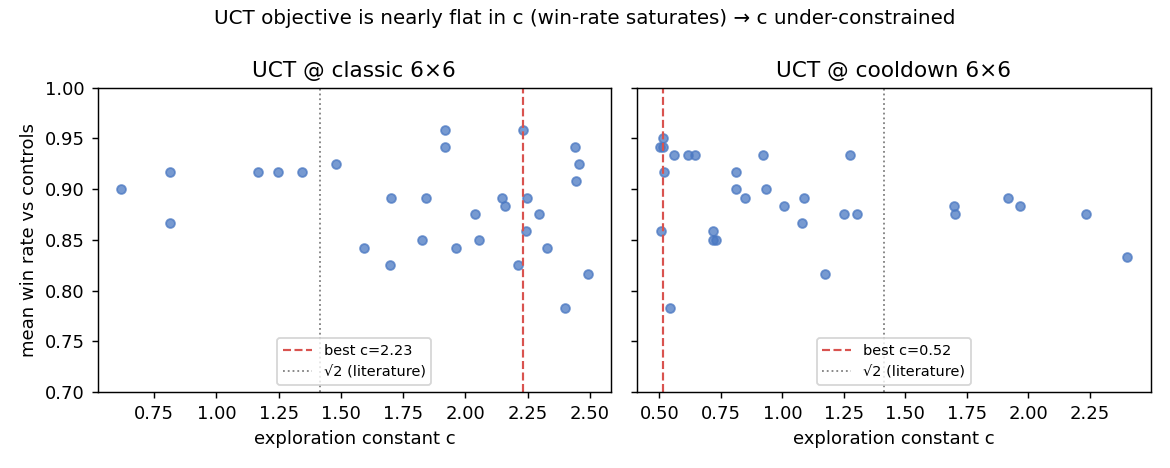
\includegraphics[height=0.6\textheight]{../05-analysis/figures/tuning_uct_c_sensitivity.png}\\
{\small Cel niemal płaski w~$c$ (klasyk) -- UCT przytłacza zestaw kontrolny, więc $c$ jest słabo
ograniczone; pod regułą stygnięcia łagodna preferencja małego~$c$. Strojenie dla silnych graczy
było \emph{co najwyżej neutralne}.}
\end{frame}

% --------------------------------------------------------------------
\begin{frame}{Weryfikacja hipotez}
\begin{itemize}
  \item[\textbf{H1}] \textcolor{green!50!black}{\textbf{potwierdzona}} -- UCT wygrywa z~Naive-Buro
        88\% (Cooldown) vs 77\% (klasyk); przewaga o~$\sim$11~p.p.\ większa pod regułą.
  \item[\textbf{H2}] \textcolor{red!70!black}{\textbf{odrzucona}} -- PB daje tylko $\sim$4~p.p.;
        UCT-PB-naive wręcz \emph{przegrywa} z~bazowym UCT.
  \item[\textbf{H3}] \textcolor{red!70!black}{\textbf{odrzucona}} -- Cooldown-Buro lepsza
        w~\emph{obu} wariantach (100\% Cooldown, $+$26~p.p.\ klasyk), nie tylko pod regułą.
  \item[\textbf{H4}] \textcolor{green!50!black}{\textbf{potwierdzona}} -- przewaga drugiego gracza
        58\% (klasyk) $\to$ 49\% (Cooldown): strukturalna przewaga \emph{znika} pod regułą.
\end{itemize}
\end{frame}

% --------------------------------------------------------------------
\begin{frame}{Eksperyment człowiek--komputer}
\small Nieformalny test: trzech graczy, po cztery partie przeciw każdemu z~trzech przeciwników
z~aplikacji webowej (wariant stygnięcia). Najsilniejszego agenta nie pokonał \emph{nikt}.
\begin{columns}[c]
\begin{column}{0.52\textwidth}\centering\scriptsize
\begin{tabular}{lccc}
\toprule
Gracz & Random & Cooldown-Buro & UCT-PB-cd \\
\midrule
Osoba 1 & 3--1 & 1--3 & 0--4 \\
Osoba 2 & 4--0 & 3--1 & 0--4 \\
Osoba 3 & 2--2 & 0--4 & 0--4 \\
\bottomrule
\end{tabular}\\[3pt]
{\scriptsize rekord \emph{wygrane--przegrane} (po 4 partie)}
\end{column}
\begin{column}{0.48\textwidth}\centering
\begin{tikzpicture}
\begin{axis}[ybar, bar width=5pt, width=\linewidth, height=4.6cm,
  symbolic x coords={Random,Cooldown-Buro,UCT-PB-cooldown}, xtick=data,
  x tick label style={rotate=18,anchor=east,font=\scriptsize}, enlarge x limits=0.30,
  ymin=0, ymax=112, ytick={0,25,50,75,100}, ylabel={wygrane [\%]},
  ylabel style={font=\scriptsize}, y tick label style={font=\scriptsize}, ymajorgrids,
  tick align=outside, nodes near coords,
  every node near coord/.append style={font=\tiny},
  nodes near coords={\pgfmathprintnumber[precision=0,fixed]{\pgfplotspointmeta}},
  legend style={font=\tiny, at={(0.5,1.03)}, anchor=south, legend columns=3}]
\addplot[fill=blue!55] table[x=opponent,y=Osoba1]{\figpath/human_winrate.dat};
\addplot[fill=teal!70] table[x=opponent,y=Osoba2]{\figpath/human_winrate.dat};
\addplot[fill=orange!75] table[x=opponent,y=Osoba3]{\figpath/human_winrate.dat};
\legend{Osoba 1,Osoba 2,Osoba 3}
\end{axis}
\end{tikzpicture}
\end{column}
\end{columns}
\vspace{2pt}
{\small Wniosek jakościowy: gra jest trudna dla początkujących -- reguła stygnięcia podnosi próg
wejścia (trzeba pamiętać, które pionki są chwilowo chronione).}
\end{frame}

% --------------------------------------------------------------------
\begin{frame}{Wnioski}
\begin{itemize}
  \item Najsilniejszy gracz: UCT-PB-cooldown -- ale główny zysk pochodzi z~samego MCTS,
        nie z~progressive bias.
  \item Reguła stygnięcia realnie zmienia grę i~mocno karze ,,naiwne'' bicia
        (zapaść Naive-Buro pod regułą).
  \item Zaskoczenie: heurystyka świadoma reguły pomaga \emph{także} w~klasycznym Othello --
        ,,trwałość bicia'' to ogólnie wartościowy sygnał.
  \item Reguła zmienia balans: znika przewaga drugiego gracza -- gra staje się bardziej
        zrównoważona, ale trudniejsza dla człowieka.
\end{itemize}
\vspace{6pt}
\centering\small Kod: \texttt{github.com/wojtke/cooldown-othello-mcts} \quad|\quad
Gra: \texttt{wojtke.github.io/cooldown-othello-mcts}
\end{frame}

\begin{frame}\centering\Large Dziękuję za uwagę\end{frame}

\end{document}
